%
%~~
%~~ Arquitetura do sistema
%~~
%


\chapter{Arquitetura do sistema}
\label{chp:arquitetura}

A arquitetura geral do sistema, incluindo todos os seus componentes, � apresentada na figura \ref{fig:arquitetura}.

\begin{figure}[htp]
	\centering
	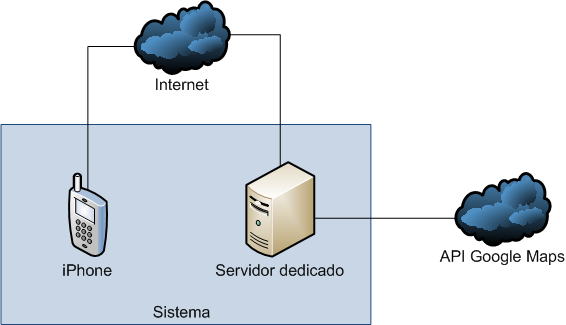
\includegraphics[scale=0.5]{img/arquitetura.png}
	\caption{Arquitetura do sistema}
	\label{fig:arquitetura}
\end{figure}

A arquitetura est� dividida basicamente em duas camadas f�sicas: 

\textbf{Servidor de aplica��o e banco dados:} Respons�vel por armazenar e disponibilizar os dados persistentes enviados pelos usu�rios do \emph{BetterWay} via internet e utilizados pelo sistema de tr�nsito. A partir dos dados, manipula a requisi��o com a \emph{API Google Maps} para gerar uma melhor rota para o dispositivo com o aplicativo. Tamb�m fornece o resultado da manipula��o dos dados para a exibi��o da malha do tr�fego atual.

\textbf{Cliente (aplica��o \emph{BetterWay}):} N� referente aos usu�rios acessando e utilizando a aplica��o \emph{BetterWay}. Na aplica��o est� a interface que apresenta o mapa com todas informa��es disponibilizadas pelo servidor. Possui um sistema interno para gerir endere�os recentes buscados, favoritos e tamb�m de informar eventos.

%%% Local Variables: 
%%% mode: latex
%%% TeX-master: "tese"
%%% x-symbol-8bits: t 
%%% End: 